\documentclass{article}
\usepackage{babel}
\usepackage[a4paper, top = 20mm, bottom=20mm, right=20mm, left=20mm]{geometry}
\usepackage{graphicx}
\usepackage{amsmath}
\usepackage{wrapfig}
\usepackage{xcolor}
\usepackage[hidelinks]{hyperref}
\usepackage{listingsutf8}
\usepackage{tocloft}
\setlength{\parindent}{3mm}
\setlength{\parskip}{5mm}
\linespread{1.65}
\renewcommand{\figurename}{Fig.}

\title{Sistemas de Información y Telemedicina II\thanks{\href{https://www.upv.es/titulaciones/GIB/indexc.html}{Grado en Ingeniería Biomédica, Escuela Técnica Superior de Ingenieros Industriales, Valencia, España.}} \\\textbf{Machine Learning para Mesotelioma Maligno}}
\author{
\href{mailto:irgarga4@etsii.upv.es}{Irene Estela García García}
\and
\href{mailto:ilcarjuc@etsii.upv.es}{Ilán Francisco Carretero Juchnowicz}
\and
\href{mailto:igamher@etsid.upv.es}{Ignacio Maria Amat Hernández}
}
\date{\today}

\lstset{
	language=Python,
	inputencoding=utf8/latin1,
	frame=single,
	numbers=left,
	basicstyle=\linespread{1.1}\ttfamily,
	mathescape,
	numberstyle=\color{gray},
	stringstyle=\color[HTML]{933797},
	commentstyle=\color[HTML]{228B22}\sffamily,
	emph={[2]from,import,pass,return}, emphstyle={[2]\color[HTML]{DD52F0}},
	emph={[3]range}, emphstyle={[3]\color[HTML]{D17032}},
	emph={[4]for,in,def}, emphstyle={[4]\color{blue}},
	showstringspaces=false,
	breaklines=true,
	prebreak=\mbox{{\color{gray}\tiny$\searrow$}},
	captionpos=b,
}


\newcommand{\diagram}[2]{
\subsubsubsection{#2}
\begin{figure}[h]
\centering
\includegraphics[width = 0.9\linewidth]{#1}
\caption{#2.}
\end{figure}
}

\newcommand{\incpng}[2]{
\begin{figure}[h]
\centering
\includegraphics[trim=3cm 3cm 3cm 0cm, width = 0.77\linewidth]{#1}
\caption{#2}
\end{figure}
}

\newcommand{\subsubsubsection}[1]{\paragraph{#1}\mbox{}\\}
\setcounter{secnumdepth}{4}
\setcounter{tocdepth}{4}
\begin{document}
\maketitle
\newpage
\tableofcontents
\listoffigures
\lstlistoflistings
\newpage

\section{Contexto y motivación}


El mesotelioma maligno (MM) es un tumor agresivo que comúnmente afecta
a las superficies mesoteliales de las cavidades pleural  y  peritoneal
y, ocasionalmente, a la túnica vaginal y el  pericardio.   Hasta  hace
poco  era  considerada	como  una  enfermedad	rara,	sin   embargo,
últimamente su incidencia está aumentando en múltiples	países	debido
al uso de asbestos, también conocido como amianto, generalmente en  el
entorno de la construcción durante la segunda mitad del siglo XX.   Se
trata de  un  carcinógeno  reconocido  por  la	OMS  desde  1987.   La
incidencia está alcanzando su punto máximo durante los	últimos  años,
reflejando el largo periodo de latencia (superior a 25 años) entre  la
exposición al amianto y el desarrollo del cáncer. Este hecho justifica
que la incidencia sea desigual en diferentes países del mundo  ya  que
depende del momento en el  que	dejó  de  usarse  el  asbesto  en  los
diferentes  países.   En  España  se  prohibió	el  asbesto  de  forma
definitiva en 2020 por lo que se espera todavía un incremento  de  los
casos hasta el año 2040. Existe un aumento progresivo a nivel nacional
de la mortalidad por mesotelioma, de 491 casos en el periodo  de  1976
al 1980 hasta los 1391 que se estima entre 2016-2020 (264 casos/ año),
un  60\%  más  que  hace  30  años.   Debido  a  las   características
epidemiológicas del MM y en especial su alta tasa  de  mortalidad,  ha
sido objeto de múltiples estudios.  Un estudio publicado en la revista
Industrial Health constata que las arcas públicas españolas sufragaron
entre  2004  y	2011,  464  millones  de  euros  para  tratar  tumores
relacionados con el amianto.

Por otra parte, el  diagnóstico  de  esta  enfermedad  puede  resultar
difícil, pues se  requiere  a  menudo  de  un  diagnóstico  patológico
realizado por un patólogo experimentado  para  diferenciar  el	MM  de
otros procesos benignos o malignos.  Además, el MM  es	un  cáncer  de
difícil terapia, hoy en día sigue siendo principalmente paliativa. Por
lo regular, no existe una cura, a menos que la enfermedad  se  detecte
muy temprano y el  tumor  se  pueda  extirpar  completamente  mediante
cirugía.  La mayoría de las veces,  al	momento  del  diagnóstico,  la
enfermedad    está    demasiado    avanzada    para    una    cirugía.

Por ello, se necesita más investigación para avanzar en  las  opciones
terapéuticas  para   el   MM,	y   estrategias   para	 realizar   la
personalización  de  la  terapia  a  través  del   descubrimiento   de
marcadores  predictivos.   Así,  el  MM  se   trata   de   un	cáncer
potencialmente	prevenible  y  predecible,  ventaja  que  se  pretende
explotar en el presente  trabajo,  con	el  fin  de  proporcionar  una
herramienta útil para la  prevención  y  diagnóstico  temprano	de  la
enfermedad, que en último término resultaría en una mayor probabilidad
de cura vía cirugía.

Para explotar esta característica de predictibilidad, una  herramienta
útil son  los  CDSS  (Clinical	Decision  Support  System),  programas
diseñados para ayudar al  profesional  de  la  salud  en  la  toma  de
decisiones clínicas, constituyen uno de los temas mas  importantes  en
el campo de la inteligencia artificial en medicina.  Muchas decisiones
en salud hoy en día son tan complejas que han sobrepasado la capacidad
de la mente humana para operar sin ayuda. El mayor desafío es tomar la
información adecuada y aplicarla a cada paciente en el momento en  que
la información sea necesaria, y dada  la  inmensa  cantidad  de  datos
clínicos de la que se dispone en la actualidad, esto se  convierte  en
una tarea imposible de llevar a cabo por un profesional por sí	mismo.
Estos sistemas computarizados, sin embargo, son capaces  de  tener  en
cuenta toda la información disponible haciendo posible la detección de
cambios fuera del alcance del profesional clínico.

A pesar de que los sistemas de ayuda a la decisión clínica
definitivamente pueden aportar beneficios con el uso de la ciencia de
datos clínicos en la práctica clínica diaria, en términos de calidad
de la atención sanitaria \cite{Belard2016}, su tasa de integración en lo relativo a los
procesos de atención clínica aún es escasa \cite{Fons}. Aún así, son sistemas con
un prometedor potencial y con muchas mejoras inminentes en el ámbito
clínico por delante, pues disponer de CDSS ha demostrado ser una de
las intervenciones más efectivas de la informática biomédica en la
mejora de la calidad asistencial y la seguridad de los pacientes.

El uso de métodos de inteligencia artificial en el diagnóstico médico
ha ido aumentando gradualmente.No hay duda de que las evaluaciones de
los datos tomados de los pacientes y las decisiones de los expertos
son los factores más importantes en diagnóstico. Sin embargo, por las
razones expuestas, a menudo son necesarias diferentes técnicas de
inteligencia artificial para clasificar una enfermedad. Así, el
diagnóstico de la enfermedad MM es una cuestión de clasificación
importante que involucra datos diversos y de diferentes fuentes, por
lo que estas técnicas podrían resultar de gran ayuda.

\begin{figure}[h]
\centering
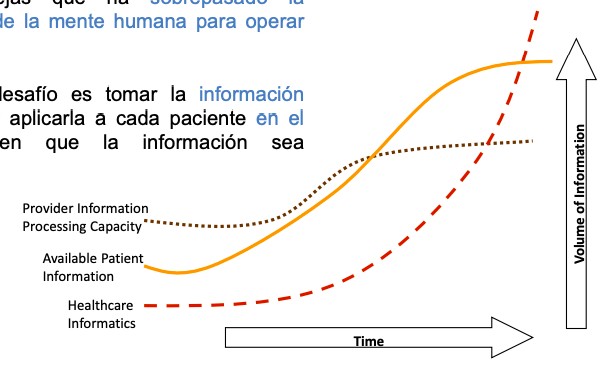
\includegraphics[width = 0.8\linewidth]{../images/cap2.png}
\caption{Incremento de información con el tiempo.}
\end{figure}

Por otra parte, otra herramienta útil para la monitorización y
seguimiento de los pacientes, así como para la prevención vía
promoción de buenos hábitos o la interacción paciente-médico o
paciente-paciente, son las aplicaciones móvil. Hoy en día, la
penetración del teléfono móvil inteligente en la población crece año
tras año, siendo el dispositivo tecnológico con mayor penetración en
países desarrollados como es España, superando ya desde hace unos años
al PC (\hyperref[fig:cap]{\textbf{Fig.}~\ref*{fig:cap}}), según el estudio de Deloitte de 2017
\cite{deloitte2017}. Según datos del informe anual Mobile Economy de
la GSMA, la población mundial que posee un móvil inteligente alcanzó
en 2017 el 57\% del total y se prevé que alcance el 77\% en 2025.

\begin{figure}[h]
\centering
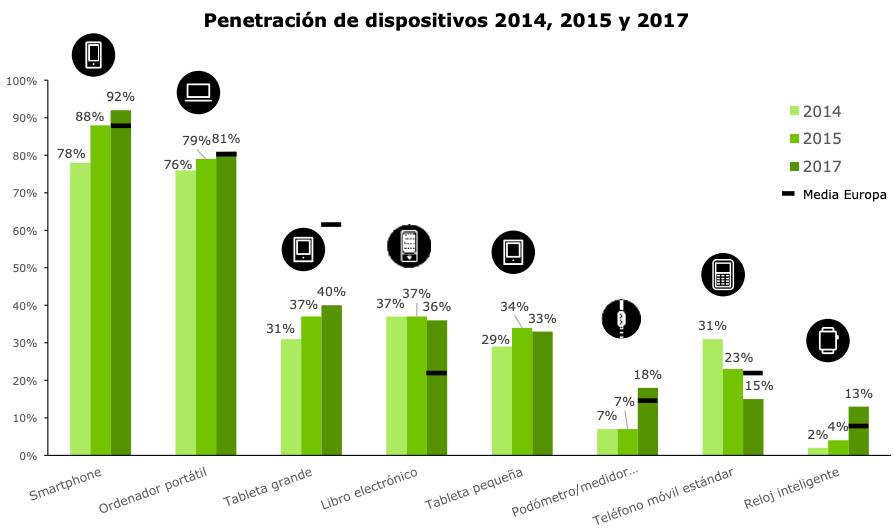
\includegraphics[width = 0.8\linewidth]{../images/cap1.png}
\caption{Global Mobile Consumer Survey.}
\label{fig:cap}
\end{figure}

Las aplicaciones son la forma favorita para conectarse desde los
dispositivos móviles: casi el 90\% del tiempo de conexión se destina al
uso de aplicaciones, y los españoles tienen una media de 16 apps
instaladas en su Smartphone. En cuanto a las apps en salud, son la
categoría de crecimiento más rápido, tanto en Android como en IOS. En
este contexto, el desarrollo de una app para el paciente de MM podría
aportar beneficios muy diversos en aspectos como pueden ser su
seguimiento y control de la evolución, hasta su potenciación como
personaje proactivo en su propia salud, así como en materia de
prevención para pacientes sanos o de riesgo.


\section{Objetivos}


En este trabajo se presenta una propuesta compuesta por varias
herramientas con el objetivo conjunto de proporcionar un marco más
favorable de la enfermedad del mesotelioma maligno, desde los puntos
de vista de la prevención, predicción y control de la evolución.

Por una parte, se ha realizado un análisis exploratorio de la base de
datos y un análisis de los factores de riesgo más significativos a la
hora de diagnosticar el MM, mediante técnicas de extracción de
características. Así, sobre este conocimiento de los datos se ha
desarrollado un modelo predictivo junto con una interfaz de usuario
amigable, para servir como CDSS en el hospital, dirigido a los médicos
como usuarios, con el objetivo de facilitar el diagnóstico prematuro,
crucial para incrementar la probabilidad de supervivencia de los
enfermos.

Por otra parte, se propone una aplicación móvil dirigida a pacientes.
Ésta tiene dos usuarios diana diferenciados. En primer lugar,
pacientes enfermos para control de la evolución del MM, permitiendo un
seguimiento más exhaustivo y de forma cómoda y remota, así como
proporcionando un marco de información fiable acerca de la enfermedad,
con posibilidad de interactuar tanto con médicos como con otros
pacientes en su misma condición. En segundo lugar, se dirige a
pacientes sanos y de riesgo, para control de los factores de riesgo de
la enfermedad y para prevención con screening y promoción de buenos
hábitos. Se ha desarrollado un prototipo de la aplicación propuesta.

Así, ambos productos finales, CDSS con interfaz para médicos y
aplicación móvil para pacientes, ambos con sus objetivos individuales,
pretenden en conjunto introducir una mejora en el marco del MM, con
objetivo último de reducir el impacto de la enfermedad y mejorar la
calidad asistencial proporcionada con respecto a ésta, así como
potenciar el papel proactivo del paciente en su salud.


\newpage
\section{Materiales y métodos}
\subsection{Base de datos}

Para realizar el trabajo, se ha utilizado la base de datos
Mesothelioma disease data set. Ésta fue preparada en la Facultad de
Medicina de la Universidad Dicle en Turquía, a partir de informes de
pacientes tomados por el médico en un hospital, contando con 324
pacientes. Todas las muestras tienen 34 variables, pues según
indicaciones de profesionales clínicos este conjunto es más eficaz que
otros subconjuntos posibles. Estas variables son edad, género, ciudad,
exposición al asbesto, tipo de MM, duración de la exposición al
asbesto, método de diagnóstico, ‘keep side’, citología, duración de
los síntomas, disnea, dolor en el pecho, debilidad, hábito de fumar,
estado funcional, recuento de glóbulos blancos (WBC), hemoglobina
(HGB), recuento de plaquetas (PLT), sedimentación, deshidrogenasa
láctica de la sangre (LDH), fosfatasa alcalina (ALP), proteína total,
albúmina, glucosa, deshidrogenasa láctica pleural, proteína pleural,
albúmina pleural, glucosa pleural, muerto o no, derrame pleural,
grosor pleural en la tomografía, nivel de acidez pleural (pH),
proteína C reactiva (PCR), clase de diagnóstico.


\subsection{Análisis exploratorio, Extracción de características y Desarrollo y evaluación de modelos.}

Para llevar a cabo todas las tareas de análisis exploratorio de los
datos, extracción de características y desarrollo y evaluación de los
modelos de predicción de MM, se han utilizado las librerías comunes
para tratamiento de datos en Python. Python se ha establecido como el
lenguaje de programación más utilizado en ciencia de datos, pues
además de ser de código abierto, proporciona todas las herramientas
necesarias para llevar a cabo estos procesos de manera efectiva y
relativamente sencilla, con poderosas bibliotecas dedicadas a ello,
algunas de las cuales, las principalmente empleadas, se describen a
continuación. Estas herramientas son idóneas para nuestro desarrollo
concreto, que requiere implementaciones muy especializadas, por lo que
las funciones básicas de estas librerías nos permiten llevar a cabo
nuestra tarea de manera muy simple y rápida.

\begin{itemize}
\item
Scikit-learn\cite{scikit-learn}: es una de las librerías más útiles para el desarrollo
algorítmico y el análisis exploratorio de datos en Python. Presenta
una amplia gama de algoritmos de aprendizaje automático para problemas
tanto supervisados, como es nuestro caso, como no supervisados, así
como métodos para la validación de los modelos, proporcionando
diferentes métricas para evaluar su desempeño.\cite{wijnhoven2019}

\item
Pandas: se trata de un paquete de Python para trabajar con dataframes
con soporte para leer y escribir datos en diferentes formatos como csv
para ser utilizados posteriormente por los modelos de clasificación.\cite{pandas}


\item
Matplotlib: se utiliza para la creación y visualización de los
		resultados gráficos, disponiendo de un amplio abanico
		de opciones.\cite{mpl}

\end{itemize}

La naturaleza open source de las herramientas empleadas para la
implementación permiten junto con github trabajar varios
desarrolladores fácilmente de forma simultánea en el proyecto.
Además, Python tiene pip, un sistema de gestión de paquetes utilizado
para instalar y administrar paquetes de software, lo que permitiría
distribuir nuestra aplicación de forma accesible si esa fuera nuestra
intención.

En cuanto a los modelos, se ha experimentado con diversos tipos,
muchos de ellos conocidos para nosotros pues los hemos estudiado en
asignaturas previas como SIT I o Imágenes Biomédcas, para poder hacer
una comparativa y seleccionar el modelo óptimo para nuestro caso de
estudio. A continuación se describen brevemente las distintas técnicas
de aprendizaje utilizadas.

\begin{itemize}
\item
LDA (Linear Discriminant Analysis) es una generalización del
discriminante lineal de Fisher, un método que trata de encontrar una
combinación lineal de las variables que separe las clases. Se trata
del modelo más simple, un modelo lineal, utilizado como primera
aproximación para observar el comportamiento de los datos y poder
comparar después con clasificadores más complejos. También se prueba
su variante QDA (Quadratic Discriminant Analysis) en la que se estima
una matriz de covarianza individual para cada clase de observaciones.
El LDA y el QDA son dos clasificadores clásicos, con, como lo sugieren
sus nombres, una superficie de decisión lineal y una cuadrática,
respectivamente. Estos clasificadores son atractivos porque tienen
soluciones de forma cerrada que pueden calcularse fácilmente, han
demostrado funcionar bien en la práctica y no tienen hiperparámetros
para ajustar.\cite{scikit-learn}

\item

KNN (K-Nearest Neighbour) es un algoritmo de clasificación supervisado
simple que podemos usar para asignar una clase a un
nuevo punto de datos. KNN no hace suposiciones sobre
la distribución de datos, por lo tanto, no es
paramétrico. Almacena todos los datos de entrenamiento
para hacer predicciones futuras al calcular la
similitud entre una muestra de entrada y cada
instancia de entrenamiento. Se trata de nuevo de un
modelo sin mayor complejidad, pero ampliamente
utilizado por ser rápido y en ocasiones suficiente.
\item

Otra técnica empleada es SVM (Support Vector Machines), un
conjunto de métodos de aprendizaje supervisado
utilizados entre otras tareas, para la clasificación.
Una de las ventajas que hacen esta técnica atractiva
para nuestro caso es que resulta bastante efectivo en
espacios de altas dimensiones, como podrían
considerarse nuestros datos con 34 variables.\cite{scikit-learn}

\item
También se ha empleado Random Forest, un meta estimador que se ajusta
		a varios clasificadores de árboles de decisión en
		varias submuestras del conjunto de datos y utiliza el
		promedio para mejorar la precisión predictiva y
		controlar el sobreajuste.

\item

PNN (Probabilistic Neural Network): una red neuronal unidireccional
		derivada de la red bayesiana y un algortítmo
		estadístico llamado Kernel Fisher discriminant
		analysis. Ha demostrado dar buenos resultados en
		estudios en el campo biomédico, por ejemplo, para
		diagnóstico clínico.\cite{Wang2010}

\item

 MLP (Multilayer Perceptron): se trata de una red neuronal que dado un
		conjunto de variables, aprende una función de mapeo no
		lineal para clasificación.

\end{itemize}

\subsection{Desarrollo Interfaz de usuario CDSS}

Para el desarrollo de la interfaz de usuario (GUI) del CDSS para ser
utilizada por el médico en el hospital para diagnóstico de MM, hemos
empleado Qt, un framework multiplataforma orientado a objetos
ampliamente usado para desarrollar software con interfaz gráfica de
usuario. Qt es de software libre y de código abierto, es flexible,
presenta muchas opciones de personalización y dispone de los widgets
apropiados y de interfaz gráfica para diseñar nuestra interfaz.
Además, la implementación en Python es simple y fácil de usar,
permitiendo una programación relativamente rápida e intuitiva. Qt
admite también otros lenguajes de programación, pero al haber elegido
Python para desarrollar los modelos, la integración es inmediata.

\subsection{Desarrollo App pacientes}

En el presente trabajo, únicamente se implementará un prototipo de la
aplicación móvil con MIT App Inventor, un entorno de programación
visual e intuitivo que permite a todos crear aplicaciones funcionales
para Smartphone y Tablet. Se ha seleccionado esta herramienta por su
facilidad de uso y rapidez de desarrollo, gracias a su filosofía de
programación basada en bloques.

Para el desarrollo de la app de la solución ideal con funcionalidad
completa, sería conveniente emplear Android Studio, el entorno de
desarrollo integrado (IDE) oficial para el desarrollo de apps para
Android.



\subsection{Servidores y conexiones y seguridad}


En lo concerniente a los servidores para almacenar la información,  se
ha decidido optar por la opción de un servidor en la  nube.   Así,  el
motivo de esta decisión reside en las ventajas que ofrece un  servidor
con estas características, ya  que  podríamos  ampliar	o  reducir  el
espacio disponible de forma flexible aumentando la rentabilidad frente
a almacenamientos compartidos o  locales.   A  su  vez,  la  idea  del
proyecto sería intentar expandir  su  alcance  a  nivel  autonómico  o
nacional progresivamente, por lo  que  sería  necesario  almacenar  la
información de los pacientes en un espacio al  que  se	pueda  acceder
fácilmente por todos los hospitales o centro sanitarios implicados  en
el proyecto sin comprometer por  ello  los  recursos  individuales  de
alguno de ellos.  A su vez, habría que optar por  una  plataforma  que
ofreciese unos umbrales de seguridad  aptos  para  el  tratamiento  de
información sanitaria, de forma  que  realmente  pudiese  aprovecharse
ventajas como la confiabilidad o escalabilidad de los servidores en la
nube.

Asimismo, incidiendo en el aspecto de la  seguridad,  el  proyecto  en
cuestión apuesta por un paciente activo el cual tiene la capacidad  de
participar activamente en su propia salud, en este  caso  mediante  la
información y recomendaciones ofrecidas en la aplicación y a partir de
la consulta de registros médicos y envío de datos de su estado	actual
a los servidores mencionados anteriormente. También, sería mencionable
que la aplicación  dispondría  no  sólo  de  un  chat  para  comunicar
pacientes, sino también para contactar con  profesionales  sanitarios,
por lo que se estaría transmitiendo continuamente información personal
y confidencial.  Por tanto, debido al flujo de datos  que  se  estaría
dando y a la condición de éstos, sería necesario el  uso  de  una  red
privada virtual (VPN).	Así, el tráfico  de  datos  generado  viajaría
cifrado, dificultando que agentes externos puedan robar la información
confidencial  transmitida.   A	su  vez,  todos  los  usuarios	de  la
aplicación podrían emplearla haciendo uso de  redes  Wi-Fi  locales  o
públicas con la tranquilidad de que se están empleando	recursos  para
proteger la integridad y  confidencialidad  de	la  información.   Por
tanto,	podríamos  emplear  protocolos	como  Ipsec  para  mejorar  la
seguridad  de  nuestras   conexiones   y   transmisiones   de	datos.

\subsection{Proyecto ALERT}

Con el fin de localizar aquellas regiones en la que la	exposición  al
asbesto fuese mayor, se emplearía el dispositivo ALERT.  Este  sistema
desarrollado como un proyecto europeo en el que han colaborado	varios
centros de investigación entre los que podríamos destacar el Instituto
de Biomecánica de Valencia (IBV), permite  detectar  la  presencia  de
fibras de amianto en el aire analizando los patrones  de  luz  de  las
partículas suspendidas en el  entorno.	 Así,  gracias	a  su  pequeño
tamaño, lo que hace que se considere un  dispositivo  portable,  junto
con la capacidad de analizar en tiempo real la cantidad de microfibras
de amianto en el espacio que lo rodea, permitiría identificar aquellas
industrias donde le riesgo fuese mayor	pudiendo  obtener  información
espacial sobre las  zonas  donde  el  nivel  de  riesgo  debido  a  la
manipulación del amianto es mayor.

\section{Resultados y discusión}
\subsection{Resolución ideal}

Con el objetivo  de  ofrecer  un  servicio  que  sea  de  utilidad  en
múltiples vertientes en lo concerniente al tratamiento del mesotelioma
maligno, se debe desarrollar dos productos que	a  su  vez  se	hallen
interconectados,  pudiendo  ofrecer  grandes  mejoras  tanto   en   la
eficiencia del hospital como en la calidad asistencial que el paciente
recibe del centro médico.

En primer lugar, se implementaría un sistema de ayuda  a  la  decisión
médica en el cual, a partir de datos a los que previamente se les haya
realizado un análisis exploratorio, se entrenarían varios  modelos  de
predicción aplicando  el  aprendizaje  supervisado  como  podrían  ser
modelos lineales, modelos  cuadráticos,  k-vecinos  o  random  forest.
Asimismo, una vez entrenados y analizadas sus métricas	de  acierto  y
error, se procedería a seleccionar el modelo que mejor resultados haya
obtenido, siempre y cuando supere unos mínimos umbrales.   Finalmente,
se dotaría al sistema de ayuda a la decisión médica en cuestión de una
interfaz amigable e intuitiva para el personal sanitario, de forma que
pudiesen a partir de la carga de datos de  un  paciente,  ejecutar  el
modelo y obtener en un tiempo reducido si el modelo considera en  base
a dichos datos si el paciente es enfermo o  sano,  ayudando  de  forma
directa al diagnóstico que realizará el médico.

En segundo lugar, se realizaría una aplicación móvil, a partir	de  la
cual mediante un sistema de usuarios y	contraseñas  pudiesen  acceder
profesionales sanitarios, enfermos e individuos con riesgo de contraer
este cáncer.  De esta forma, cada grupo de personas podría  acceder  a
unos servicios u otros según su condición.

Así, aquellos pacientes que padezcan el cáncer dispondrían de un  chat
con otros enfermos con el fin de recibir  apoyo  y  consejos  unos  de
otros.	También, tendrían la posibilidad de conversar con sus médicos,
y a su vez estarían  analizando  su  estado  diariamente,  ya  que  la
aplicación enviaría notificaciones en las  cuales  se  pediría	a  los
pacientes que introdujesen datos que fuesen relevantes para el estudio
de la situación del enfermo, como podría ser el dolor de  pecho  o  la
debilidad.  Cabe destacar que, también estarían  geolocalizados  y  se
identificaría en un  mapa  aquellos  puntos  donde  la	exposición  al
asbesto es mayor, y al pasar cerca  de	éstos,	la  app  emitiría  una
notificación alertando a tales enfermos,  además  de  también  alertar
sobre	las   citas   médicas	y   la	 ingesta   de	 medicamentos.

Los pacientes en riesgo dispondrían de un chat para consultarle  dudas
a sus respectivos médicos, además de tener la misma monitorización que
los pacientes enfermos,  variando  las	notificaciones	recibidas  (un
mayor número de recomendaciones sobre consejos y hábitos  a  realizar)

Finalmente,  los  médicos  tendrían  disponible  un  chat  para  poder
resolver las cuestiones que tengan  los  pacientes  de	riesgo	y  los
enfermos, e incluso poder preguntar a los pacientes que  considere  en
que estado se encuentran, pudiendo realizar un primer estudio  general
vía chat.  Cabe recalcar, que los tres grupos  de  usuarios,  médicos,
pacientes y personas en riesgo dispondrían  de	información  sobre  el
amianto,  donde   se   halla,	que   puede   ocasionar,   prevención,
concienciación y buenas prácticas.

En síntesis, si bien es verdad que el servicio se  compondría  de  dos
productos, el objetivo principal es coordinación entre ambos, de forma
que, los datos	que  se  vayan	recogiendo  de	los  pacientes	en  la
aplicación, se envíen y almacenen de forma segura en servidores a  los
que se pueda acceder desde el sistema de ayuda a la decisión  clínica,
de manera que a la hora de realizar distintas exploraciones y  obtener
nuevos análisis de los pacientes, los datos que haya podido introducir
directamente desde la aplicación el paciente  queden  ya  registrados,
acelerando  los  flujos  de  trabajo  del  hospital.   Por  tanto,  se
promociona la condición de paciente activo, donde se hace partícipe al
propio paciente del cuidado  de  su  salud,  ofreciéndole  los	medios
necesarios para mejorar su calidad de vida mediante el	tratamiento  y
prevención del mesotelioma maligno a partir del uso de las tecnologías
de la información y la comunicación.

\subsection{Resolución real}

Si bien es verdad que las implementaciones realizadas servirían a modo
de una primera aproximación de lo que podría ser un proyecto  de  esta
envergadura, podrían considerarse  de  gran  utilidad  a  la  hora  de
considerarse como prototipados, de forma que la solución real  acabara
aproximándose al máximo a la solución ideal.

En lo concerniente al sistema de  ayuda  a  la	decisión  clínica,  en
primer lugar, se ha realizado un análisis exploratorio	de  los  datos
para identificar datos	anómalos  y  aquellas  variables  que  podrían
resultar más significativas. Así, pese a tener variables de relevancia
con el mesotelioma maligno como podría ser la exposición al asbesto  o
la duración de ésta, analizando los datos disponibles en  la  base  de
datos de enfermos y sanos, observamos como como los valores de unos  y
otros son muy similares en la mayoría de campos,  por  lo  que	se  ha
descartado la idea de reducir la dimensionalidad inicialmente. Muestra
de ello puede ser los histogramas de las variables, donde  se  aprecia
que los valores de para sanos y  enfermos  son	muy  similares	en  la
mayoría de casos, o el gráfico de Pareto donde podemos visualizar como
serían necesarias 17 componentes para explicar el 80\% de la  varianza
de los datos, por lo que se concluye las componentes explican muy poca
varianza individualmente.

\vfill

\begin{figure}[h]
\centering
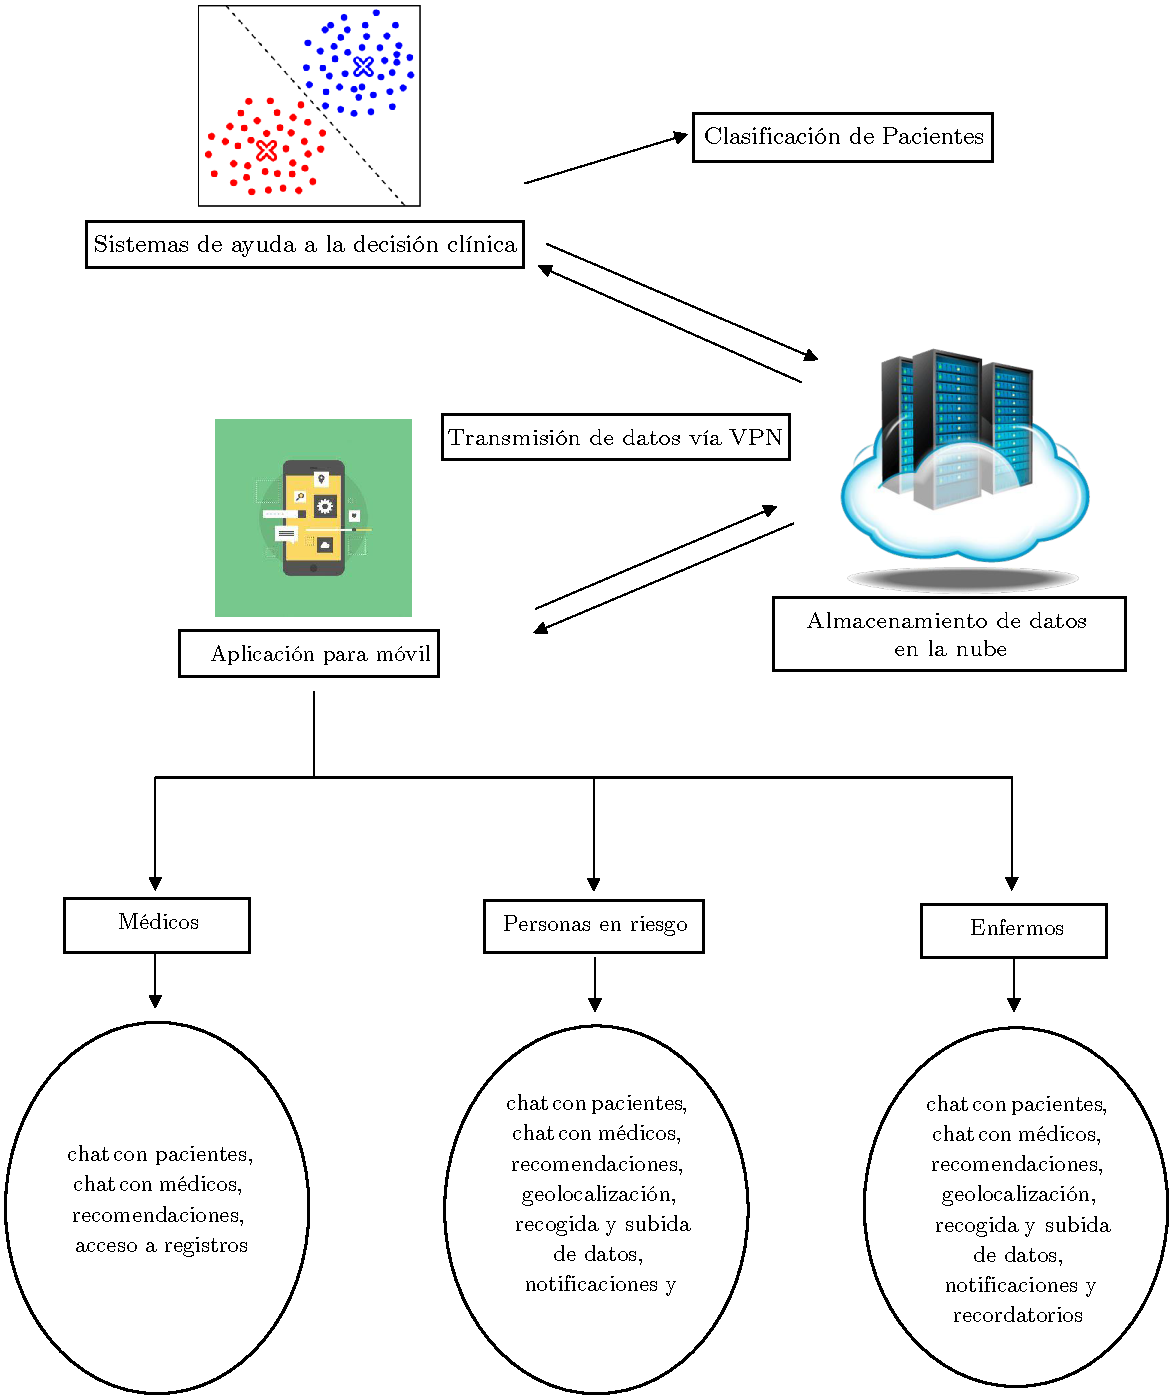
\includegraphics[width = \linewidth]{../images/esquemaideal.pdf}
\caption{Esquema teórico de la solución ideal.}
\end{figure}

\clearpage
\subsubsection{Análisis exploratorio}
\subsubsubsection{Tipos de datos}

Comenzamos analizando la base de datos,  consta de las siguientes
variables:
\begin{lstlisting}[
	label=lst:cod1,
	caption = {Variables de la base de datos.},
	]
RangeIndex: 324 entries, 0 to 323
Data columns (total 30 columns):
 #   Column                            Non-Null Count  Dtype
---  ------                            --------------  -----
 0   age                               324 non-null    float64
 1   gender                            324 non-null    int64
 2   city                              324 non-null    int64
 3   asbestos exposure                 324 non-null    int64
 4   duration of asbestos exposure     324 non-null    float64
 5   keep side                         324 non-null    int64
 6   duration of symptoms              324 non-null    float64
 7   dyspnoea                          324 non-null    int64
 8   ache on chest                     324 non-null    int64
 9   weakness                          324 non-null    int64
 10  habit of cigarette                324 non-null    int64
 11  performance status                324 non-null    int64
 12  white blood                       324 non-null    float64
 13  cell count (WBC)                  324 non-null    int64
 14  hemoglobin (HGB)                  324 non-null    int64
 15  platelet count (PLT)              324 non-null    float64
 16  sedimentation                     324 non-null    float64
 17  blood lactic dehydrogenise (LDH)  324 non-null    float64
 18  alkaline phosphatise (ALP)        324 non-null    float64
 19  total protein                     324 non-null    float64
 20  albumin                           324 non-null    float64
 21  glucose                           324 non-null    float64
 22  pleural lactic dehydrogenise      324 non-null    float64
 23  pleural protein                   324 non-null    float64
 24  pleural albumin                   324 non-null    float64
 25  pleural glucose                   324 non-null    float64
 26  pleural effusion                  324 non-null    float64
 27  pleural thickness on tomography   324 non-null    float64
 28  pleural level of acidity (pH)     324 non-null    float64
 29  C-reactive protein (CRP)          324 non-null    int64
dtypes: float64(18), int64(12)
memory usage: 76.1 KB
\end{lstlisting}

Nuestra base de datos consta de 324 entradas, cada una  con 30
variables. Todos los valores son \lstinline{floats} e
\lstinline{ints}, además no tenemos ningún \lstinline{NULL}.

\newpage
\diagram {../images/boxplot.pdf}{Caja bigotes}

Vemos que no hay diferencias notables entre los diagramas  de  nuestra
población   de	 pacientes   sanos   y	 enfermos.    Las   variables
\lstinline{PLT, PLT, glucosa} y \lstinline{PLD}  parecen  tener  datos
anómalos.

\newpage
\diagram {../images/histogram.pdf}{Histograma}

Como es de esperar tras juzgar los  diagramas  de  caja  bigotes,  los
histogramas también tienen una distribución casi idéntica. Lo único en
lo que se diferencian es  en  la  cuentas  totales,  ello  indica  que
tenemos  más  observaciones  de  pacientes  sanos  que	de   enfermos.

\newpage
\diagram {../images/kdens.pdf}{Kernel Density}

A diferencia de los histogramas, al  tratarse  con  densidades	no  se
observan diferencias por la  distinta  cantidad  de  observaciones  de
sanos y enfermos.  Únicamente vemos que las  distribuciones  son  casi
idénticas, como intuíamos de los histogramas.

\newpage
\diagram {../images/qqplot.pdf}{Cuantil - cuantil}

\newpage
\diagram {../images/corrtodas.pdf}{Correlaciones}

\newpage
\subsubsection{Extracción de Características}
\subsubsubsection{Filter methods}

\begin{lstlisting}[
	label=lst:cod2,
	caption = {Selecci\'on de variables seg\'un \lstinline{fscore}},
	]
Ranking    Variable
-------    --------
 1         pleural level of acidity (pH)
 2         C-reactive protein (CRP)
 3         gender
 4         pleural lactic dehydrogenise
 5         pleural effusion
 6         pleural glucose
 7         pleural albumin
 8         keep side
 9         blood lactic dehydrogenise (LDH)
10         total protein
11         alkaline phosphatise (ALP)
12         white blood
13         performance status
14         cell count (WBC)
15         habit of cigarette
16         pleural protein
17         duration of asbestos exposure
18         city
19         dyspnoea
20         ache on chest
21         sedimentation
22         asbestos exposure
23         platelet count (PLT)
24         glucose
25         albumin
26         duration of symptoms
27         weakness
28         age
29         hemoglobin (HGB)
30         pleural thickness on tomography
\end{lstlisting}

Usando la puntuación de \textit{Fisher} clasificamos las
características de mayor a menor relevancia a la hora de resolver el
problema de clasificación

\newpage
\subsubsubsection{Wrapper methods}
\begin{lstlisting}[
	label=lst:cod3,
	caption = {Mejores variables seg\'un \lstinline{SFS} y \lstinline{SBS}},
	]
0.6782828282828283
Sequential Forward  Selection ('asbestos exposure',
				'keep side',
				'weakness',
				'cell count (WBC)',
				'platelet count (PLT)',
				'alkaline phosphatise (ALP)',
				'glucose',
				'pleural protein',
				'pleural glucose',
				'C-reactive protein (CRP)')

0.5414285714285715
Sequential Backward Selection ('city',
			       'asbestos exposure',
			       'keep side',
			       'duration of symptoms',
			       'ache on chest',
			       'performance status',
			       'platelet count (PLT)',
			       'alkaline phosphatise (ALP)',
			       'pleural albumin',
			       'C-reactive protein (CRP)')
\end{lstlisting}

Una selección secuencial hacia adelante y hacia atrás con un modelo de
\lstinline{randomforest} con 100 estimadores y 10 parámetros
calculamos una precisión del 67\%. Los resultados son menores cuando
hacemos la selección hacia atrás. También lo hemos intentado con un
modelo \lstinline{knn}, los resultados son peores en torno al 50\%.

\subsubsubsection{PCA}

\begin{wrapfigure}[6]{l}{0.6\linewidth}
\centering
\vspace{-1cm}
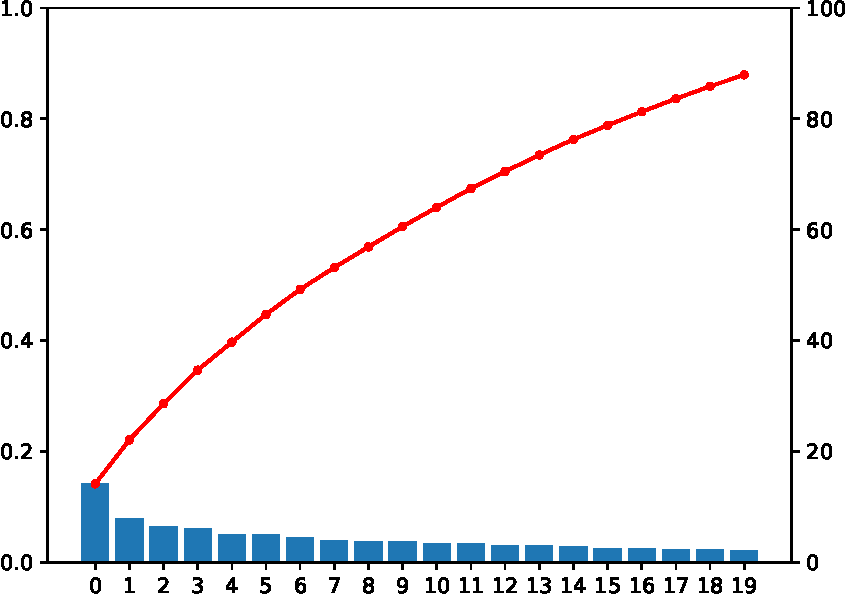
\includegraphics[width = 0.9\linewidth]{../images/pareto.pdf}
\caption{Diagrama de pareto.}
\end{wrapfigure}
Calculando el diagrama de pareto vemos que necesitaríamos entorno a 17
componentes para explicar el 80\% de la varianza de los datos. Con
estos resultados vemos que  será difícil reducir al dimensionalidad
de nuestros datos.

\newpage
\subsubsection{Modelos de Clasificación}

En segundo lugar, se ha procedido a programar varios modelos en Python
a partir de las  librerías  disponibles  para  el  desarrollo  de  tal
implementación.  Así se  ha  seleccionado  el  análisis  discriminante
lineal (LDA), el análisis discriminante cuadrático  (QDA),  k  vecinos
(KNN), random forest (RF), máquinas de soporte	vectorial  (SVM),  una
red neuronal probabilística (PNN) y un perceptrón multicapa (MLP).  De
esta forma, se han obtenido los siguientes resultados en lo relativo a
la precisión, sensibilidad, especifidad y tiempo de ejecución  de  los
respectivos modelos.


% \begin{lstlisting}[
%         label=lst:cod3,
%         caption = {Modelos de clasificaci\'on en Python},
%         ]
% from sklearn.discriminant_analysis import LinearDiscriminantAnalysis

% modeloLDA = LinearDiscriminantAnalysis ();

% from sklearn.discriminant_analysis import QuadraticDiscriminantAnalysis

% modeloQDA = QuadraticDiscriminantAnalysis ();

% from sklearn.neighbors import KNeighborsClassifier

% modeloKNN   = KNeighborsClassifier (n_neighbors = 50)

% from sklearn.ensemble import RandomForestClassifier

% modelFOREST = RandomForestClassifier (
%         n_estimators = 100,
%         criterion = 'gini',
%         )

% from neupy import algorithms

% modeloPNN = algorithms.PNN (
%         std=5,
%         verbose=False,
%         )

% from sklearn.neural_network import MLPClassifier as MLP

% modeloMLP = MLP(
%         hidden_layer_sizes = (175, 100, 50, 25, ),
%         max_iter = 500,
%         random_state = 1)

% from sklearn import svm

% modeloSVM = svm.LinearSVC()
% \end{lstlisting}

\vfill
\begin{table}[h!]
\centering
\begin{tabular}{|c|c|c|c|c|c|c|c|c|}
\hline
Model  & TP    & FP    & FN    & TN   & Accuracy & Sensitivity & Specificity & Time\\
\hline
   LDA & 58.45 & 10.60 & 21.31 & 7.63 &  0.67    & 0.73        & 0.42        & 5.21\\
   QDA & 55.93 & 12.94 & 22.43 & 6.70 &  0.64    & 0.71        & 0.34        & 4.58\\
   KNN & 68.99 & 0.00  & 29.01 & 0.00 &  0.70    & 0.70        & nan         & 9.74\\
FOREST & 66.55 & 2.54  & 23.96 & 4.95 &  0.73    & 0.74        & 0.66        & 181.79\\
   SVM & 45.93 & 22.88 & 19.88 & 9.31 &  0.56    & 0.70        & 0.29        & 20.90\\
   PNN & 61.88 & 7.06  & 25.27 & 3.78 &  0.67    & 0.71        & 0.35        & 9.15\\
   MLP & 48.57 & 20.53 & 20.42 & 8.48 &  0.58    & 0.70        & 0.29        & 287.44\\
\hline
\end{tabular}
\caption{Resultados agregados tras 1000 repeticiones.}
\label{table:}
\end{table}


\vfill

\subsubsection{Interfaz}

Asimismo, con el fin de prestar una facilidad al usuario de cara a
usar los modelos predictivos en cuestión, se han realizado dos
interfaces simples para mostrar los resultados que se deseen. La
primera interfaz desarrollada nos abre primeramente una ventana donde
podemos introducir los datos del paciente a analizar mediante el
sistema de ayuda a la decisión clínica. Asimismo, con el fin de
facilitar la introducción de datos en el sistema la interfaz permite
cargar un archivo (.csv) con todos los datos para proceder al estudio
en cuestión. Una vez, se ha comprobado que los valores introducidos
son correctos o modificado desde la propia interfaz aquellos que no lo
sean, se indica con que modelo se pretende realizar la clasificación,
mostrando en un tiempo reducido las métricas de evaluación del modelo
para la base de datos y el diagnóstico particular para los datos
introducidos (sano o enfermo). A continuación se muestra en
detalldamente la funcionalidad y la nvegación de nuestra la app.

\newpage

\vfill
\incpng{../images/s1.png} {Ventana principal.}
\vfill

Ventana principal de nuestra interfaz. A la izquierda campos de texto
para introducir las variables, se muestra entre paréntesis el rango de
dicha variable en nuestra base de datos.

\vfill
\begin{figure}[h]
\centering
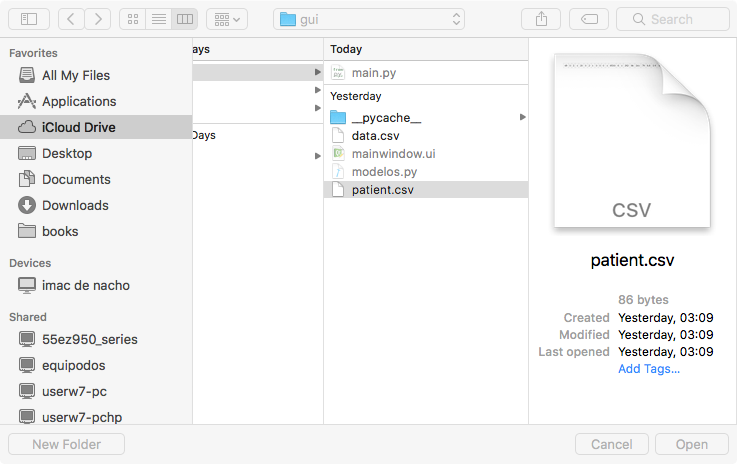
\includegraphics[trim=3cm 1cm 3cm 0cm, width = 0.5\linewidth]{../images/s2.png}
\caption{Selección de paciente.}
\end{figure}
\vfill

Para hacer mas cómodo su uso y evitar tener que introducir 30+
variables a mano, al presionar Cmd + O se abre una ventana para
seleccionar un archivo .csv, contiene todos los valores para un
paciente separados por comas.

\newpage
\incpng{../images/s3.png} {Importación paciente.}

Al importar el paciente se rellenan automáticamente las variables,  se
pueden comprobar y editar si fuera necesario.

\incpng{../images/s4.png} {Cargar variables.}

Al presionar Enter con el teclado o el botón 'Leer Vars' con el  ratón
se guardan las variables en la memoria del programa.  Para  actualizar
una variable no hay más que introducir un nuevo valor y pulsar enter o
el ratón.

Para cargar el modelo se presiona Ctrl + M, o se elige desde el menú.
Aparece una venta para seleccionar el archivo .py con los modelos en
python.

\newpage
\begin{figure}[h]
\centering
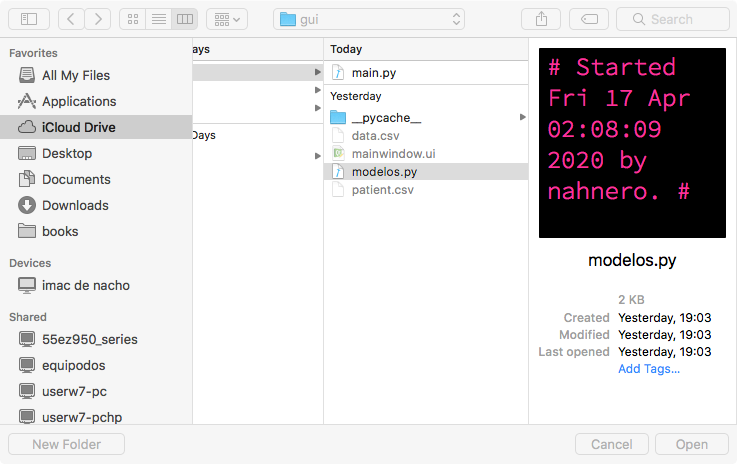
\includegraphics[trim=3cm 1cm 3cm 0cm, width = 0.5\linewidth]{../images/s5.png}
\caption{Selección de modelos.}
\end{figure}

Una vez cargados  los  modelos	se  selecciona	que  modelo  se  desea
ejecutar, los botones son mutuamente excluyentes.   Al	ejecutarse  el
modelo se generan las  métricas  de  evaluación  a  la	derecha  y  el
diagnóstico.

\incpng{../images/s6.png} {Selección de modelos.}

Cuando se selecciona otro modelo se revalúa al paciente,  cada	modelo
tiene  unas  características  diferentes  en   cuanto	a   exactitud,
sensitividad y especificidad.  En función de lo que se busque se puede
seleccionar un modelo adecuado.

Si bien es verdad que es un prototipado  básico  y  que  podría  tener
mejoras en múltiples aspectos (interfaz más amigable,  más  funciones,
pruebas  de  usabilidad...)  es  importante   recalcar	 el   objetivo
específico que se pretende con dicho interfaz en particular.  En  este
caso, estaría destinado a  una	vertiente  de  carácter  investigador,
donde se pretenda comparar los múltiples modelos  empleados,  analizar
sus resultados y determinar en que situaciones convendría utilizar  un
determinado  modelo  u	otro  según  la  distribución  de  los	datos.

No obstante, a la hora de emplear un sistema de ayuda  a  la  decisión
clínica de forma continuada y habitual en  centros  hospitalarios,  la
opción de incluir varios de modelos de predicción no es relevante,  ya
que la finalidad en este caso es simple; obtener la clasificación  del
modelo con mejores métricas para  ayudar  al  diagnóstico  médico  del
mesotelioma maligno.  Por tanto, se ha desarrollado también un segundo
interfaz donde se anula la posibilidad de  seleccionar	un  modelo  en
particular, y a partir de los datos introducidos el  modelo  clasifica
al paciente como sano o enfermo.

\subsubsubsection{Aplicación para médicos}

Esta versión restringe al usuario a usar un modelo predeterminado.
Al pulsar el botón ejecutar, después de haber introducido los datos del
paciente se calcula el modelo y se presentan los resultados.

\incpng{../images/s8.png} {Versión limitada para médicos.}


Así, aunque sería más idóneo que el modelo  clasificase  el  grado  de
enfermedad en vez de  dar  un  resultado  binario,  se	demuestra  que
perfeccionando los modelos de predicción y alimentando los modelos con
más datos podría llegarse a un sistema de ayuda a la decisión  clínica
de gran utilidad para cualquier profesional médico, ya	que  en  pocos
segundos o minutos se obtendría  una  precisión  a  tener  en  cuenta.
Asimismo, cabe destacar que también habría que consolidar una interfaz
intuitiva y amigable de forma que al personal sanitario le suponga una
mejora en su calidad y ritmo  de  trabajo  y  no  un  descenso	en  su
rendimiento habitual.


El sistema de ayuda a la decisión clínica en este caso sería  de  gran
utilidad para  diagnosticar  el  mesotelioma  maligno  prematuramente,
pudiendo ofrecer un mejor tratamiento desde un inicio.	 No  obstante,
tal y como se ha expuesto en la solución ideal, se busca una  solución
para el problema del mesotelioma maligno relación con la exposición al
amianto.  Luego entonces, únicamente realizando un prototipado	de  un
sistema de apoyo a la decisión clínica, si bien es cierto que  nuestro
proyecto sería útil,  también  se  podría  definir  como  un  proyecto
incompleto donde no se estaría optimizando los recursos existentes  en
la actualidad relacionados tanto con  las  TICS  como  con  el	propio
mesotelioma maligno.

\subsubsubsection{Aplicación para pacientes}

De esta forma, intentando aportar una solución integral a la situación
expuesta en lo referente al amianto y al mesotelioma  maligno,	se  ha
desarrollado también una primera aproximación  de  lo  que  sería  una
aplicación móvil para enfermos, personas en riesgo  y  médicos.   Así,
mediante la herramienta desarrollada por el instituto  tecnológico  de
Massachusetts  (MIT)  App  Inventor,  se  ha  podido  implementar   un
prototipado con varias de las funcionalidades de las que la aplicación
en su fase definitiva debería ofrecer.

Inicialmente al abrir la app nos encontramos con una pantalla  inicial
en la cual podemos iniciar sesión o registrarnos  como	pacientes  que
padecen la enfermedad, individuos de riesgo o  profesionales  médicos.
Así, aunque en este sistema de registro al final se termina accediendo
al mismo menú en los tres casos debido a que en la base  de  datos  se
guardan sin distinción alguna entre enfermos,  personas  en  riesgo  y
personal  sanitario,  se  ha  considerado  relevante  plasmar  en   el
prototipado la distinción entres grupos distintos de usuarios. De esta
forma, de cara a la consolidación de una aplicación sólida, habría que
guardar cada usuario con la pertenencia correspondiente al grupo en el
que se han registrado, de manera que los servicios ofrecidos  en  cada
inicio de sesión serían distintos según seamos enfermos, personas  con
riesgo o médicos.  Asimismo, la cuenta debería estar conectada con  un
identificador único, de manera que médicos  y  pacientes  tuviesen  la
posibilidad a acceder a registros personales.

Una vez, llegados al menú principal, en el caso de primera versión  de
la aplicación se nos ofrecen cinco opciones: contactar con un médico o
paciente mediante correo electrónico, visualizar nuestra  ubicación  y
las zonas donde la exposición al amianto sea  elevada,	información  y
recomendaciones sobre el problema a  tratar,  las  cuales  pueden  ser
reproducidas vía audio, con un	enlace	para  descargar  una  guía  de
prevención contra el amianto y un registro donde introducir  variables
referentes al paciente, las cuales pueden luego  almacenarse  como  un
archivo csv para luego poder enviarlas al centro médico.   A  su  vez,
pese a la precariedad del registro de datos implementado, ya que  para
enviar los datos habría que emplear otra aplicación  en  el  caso  del
prototipado  desarrollado,   incluye   varias	funcionalidades   como
renombrar variables o eliminar y modificar registros.  Finalmente,  en
el menú principal implementado también existe la opción de  volver  al
inicio, lo cual sería equivalente en este desarrollo inicial a	cerrar
sesión.

\newpage
\begin{figure}[h!]
\centering
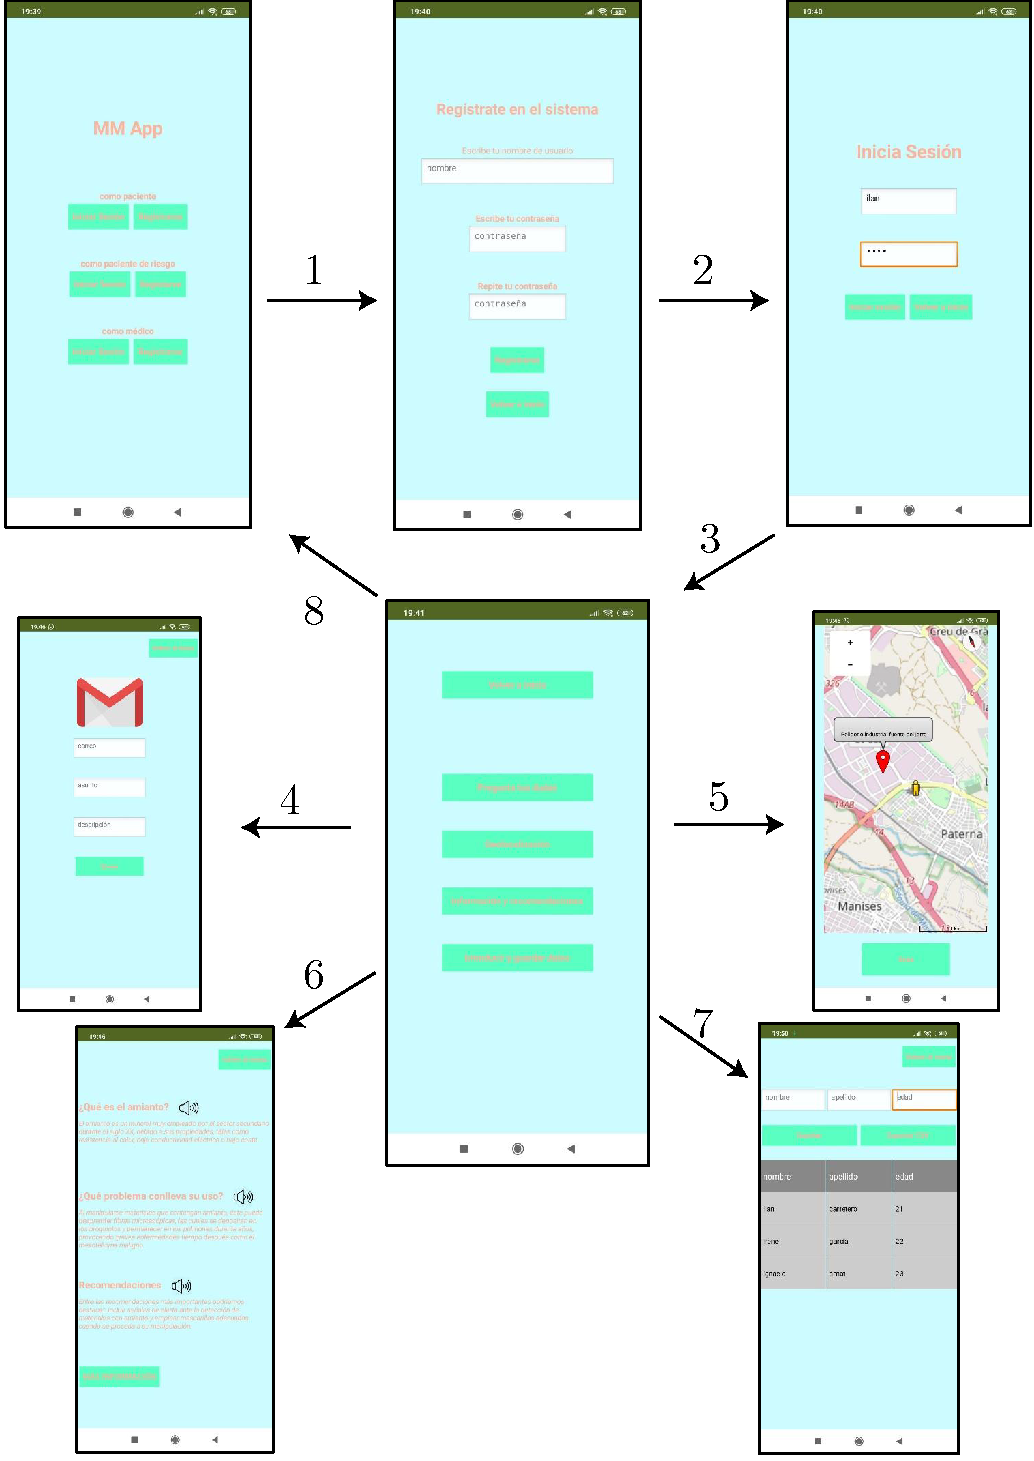
\includegraphics[width = 0.8\linewidth]{../images/esquema_aplicacion.pdf}
\caption{Esquema de la aplicación.}
\end{figure}

Por tanto, ha quedado patente la versatilidad y eficacia que  presenta
App Inventor, ya que permite el  desarrollo  del  prototipado  de  una
aplicación de forma muy simple, intuitiva a partir de nociones básicas
de programación que cualquiera	puede  aprender  muy  fácilmente.   No
obstante, pese a que se  puede	considerar  una  primera  aproximación
correcta, evidentemente es  incompleta	ya  que  carece  de  múltiples
funcionalidades  que   requerirían   sumergirnos   en	lenguajes   de
programación como C++, Java o Kotlin, para los cuales sería  necesaria
una inversión de tiempo mucho mayor. Así, para llegar a una aplicación
donde verdaderamente se sobrepasase la fase de prototipado, habría que
posiblemente emplear uno de estos lenguajes y  añadir  las  siguientes
funcionalidades principalmente:

\begin{itemize}
\item
Conexión entre las sesiones y los registros médicos, de forma que
médicos y pacientes pudiesen acceder a dichos registros

\item
Almacenar usuarios teniendo en cuenta si son profesionales sanitarios,
personas de riesgo o enfermos, de forma que los servicios existentes
en cada menú fuesen distintos

\item
Inclusión de un chat para todos los menús, de manera que los pacientes
pudiesen contactar entre ellos y con sus respectivos médicos, pudiendo
ayudarse unos a otros y disponiendo de un canal de comunicación fluido
para contactar con el personal sanitario

\item
En los servicios disponibles para médicos, eliminar la opción de
registrar datos y añadir un nuevo servicio que fuese para visualizar
los registros de los pacientes

\item
Tanto en pacientes de riesgo como enfermos, posibilitar la opción de
introducir todos los datos que precise el médico para un diagnóstico
inicial de los que pueda disponer el paciente, y subir los datos a un
servidor a partir del cual el sistema de ayuda a la decisión clínica y
otros servicios del hospital pudiesen acceder.

\item
Adición de notificaciones y recordatorios de citas, ingesta de
medicamentos y medidas de seguridad para personas de riesgo y enfermos

\item
Monitorización de la posición de los pacientes, de forma que al estar
a menos de una determinada distancia de una zona con una gran
exposición al amianto, saltase una alarma.

\item
Inclusión en el servicio de información y recomendaciones enlaces a
videos, noticias de periódico y más información que se fuese
actualizando periódicamente.
\end{itemize}

\section{Conclusiones}


La ciencia de datos tiene grandes contribuciones que ofrecer al  campo
biomédico y clínico, con los CDSS como potencial herramienta de  apoyo
a los profesionales clínicos en el análisis de la información clínica,
con la capacidad de introducir	un  incremento	de  la	mejora	de  la
calidad del servicio asistencial proporcionado a los pacientes.  En el
caso del MM, un modelo de aprendizaje supervisado tipo	Random	Forest
podría resultar de ayuda en el diagnóstico prematuro de la  enfermedad
a través de datos de pruebas clínicas y datos recopilados directamente
del paciente de forma sencilla.  Un diagnóstico precoz es esencial  en
este caso para la supervivencia del paciente.

El porcentaje de población que posee un teléfono  inteligente  aumenta
año tras año, y las apps móviles están en pleno auge, con una tasa  de
crecimiento especialmente elevada en el sector de la salud.  Esto debe
verse como una gran ventaja a ser explotada.  Las aplicaciones móviles
de salud pueden servir en un caso como el estudiado  del  MM  no  solo
para monitorizar y controlar  la  evolución  de  la  enfermedad,  sino
también   para	 prevención    y    empoderamiento    del    paciente.

El uso de diversas herramientas de TICS aplicadas al sistema sanitario
ofrecen la posibilidad de generar potenciales mejoras en  el  servicio
asistencial, siendo capaces de crear un marco  de  integración	de  la
información y procesos involucrados en un cierto caso, como el del MM,
para su mejor gestión.	Para el diseño, desarrollo e  implantación  de
tales sistemas de carácter integrador o global, es  fundamental  tanto
una correcta identificación del problema a  resolver  como  un	equipo
multidisciplinar capaz de abordar las tan diversas tareas  implicadas.

\section{Lecciones aprendidas y reflexiones}

Mediante la realización del trabajo en cuestión hemos podido comprobar
la dificultad que supone no  sólo  plantear  una  idea,  sino  también
llevarla a la práctica.  Es preciso y  fundamental  iniciar  cualquier
proyecto comprendiendo correctamente el  problema  identificado,  para
poder luego desarrollar una solución que realmente sea	útil  y  pueda
aplicarse en la resolución de aquello que se  pretende	alcanzar.   Es
precisamente  por  ello  por  lo  que  se  ha  pretendido  abordar  el
tratamiento del  mesotelioma  maligno  desde  la  perspectiva  de  las
tecnologías de la información y la comunicación  mediante  un  enfoque
global.  Con esto nos referimos a que se ha intentado prototipar de un
proyecto en el que se pretende ayudar tanto a pacientes  e  individuos
de riesgo como	a  profesionales  sanitarios,  con  el	fin  de  poder
consolidar  una   solución   integral	al   problema	en   cuestión.

No obstante, si dicho proyecto se fuese  a  realizar  para  finalmente
obtener una solución verdaderamente aplicable a los hospitales y a  la
sociedad, es evidente que se necesitaría un equipo multidisciplinar en
el  que  deberían  colaborar  médicos,	ingenieros  y  pacientes  para
realmente  identificar	aquellos  puntos   del	 problema   donde   la
utilización de recursos tecnológicos e	informáticos  permitiesen  una
mejora directa en la calidad de vida del paciente.  Asimismo,  durante
el desarrollo del trabajo expuesto se ha incidido en  el  concepto  de
paciente activo, ya que mediante el  uso  de  las  tecnologías	de  la
información y comunicación dicho paciente, en un pasado pasivo,  puede
adquirir un rol principal en el cuidado de su salud  a	partir	de  su
colaboración con el personal sanitario mediante el uso por ejemplo  de
aplicaciones móviles.

A su vez, es de vital importancia mencionar los controles que deberían
pasar todas y cada una de las partes que integran el  proyecto,  tanto
el sistema de ayuda a la decisión clínica y la aplicación móvil,  como
la seguridad en la transmisión y el almacenamiento de datos durante el
flujo de trabajo de la solución desarrollada.

Las  tecnologías  de  la  información	y   la	 comunicación	pueden
considerarse como uno  de  los	valores  más  significativos  a  nivel
actual, no sólo para  el  sector  industrial,  sino  también  para  el
mercado sanitario.   Así,  a  partir  del  acoplamiento  de  múltiples
herramientas que colaboren y actúen en sintonía unas con otras	existe
la posibilidad de mejorar y optimizar los recursos clínicos y médicos,
lo que conlleva de forma directa una mejora en la calidad  asistencial
del  protagonista  del	campo  sanitario:  el  paciente.   Finalmente,
destacar que durante la realización del trabajo se  ha	ido  aplicando
los conocimientos adquiridos durante la  carrera,  y  específicamente,
los desarrollados en las asignaturas  de  sistemas  de	información  y
telemedicina, por lo que se ha podido aplicar a la  resolución	de  un
problema  (al  menos,  en  el  planteamiento  de  la  solución	y   el
prototipado de la misma) demostrando utilidad y aplicabilidad  de  los
contenidos académicos a la realidad.


\newpage
\bibliographystyle{unsrt}
\bibliography{ref}

\end{document}
